\documentclass[10pt, usepdftitle=false]{beamer}



\newcommand\hmmax{0}
\newcommand\bmmax{0}

\usetheme[progressbar=frametitle]{metropolis}
\usepackage{appendixnumberbeamer}

\usepackage{booktabs}
\usepackage{soul}
\usepackage{csquotes}
\usepackage[scale=2]{ccicons}
\usepackage{bm}
\usepackage[export]{adjustbox}

\usepackage{style/main}
\usepackage{style/defs}

\usepackage{pgfplots}
\usepgfplotslibrary{dateplot}

\usepackage{xspace}
\newcommand{\themename}{\textbf{\textsc{metropolis}}\xspace}
\definecolor{mLightGreen}{HTML}{14B03D}
\definecolor{vpGreen}{HTML}{66c2a5}
\definecolor{vpOrange}{HTML}{fc8d62}
\providecommand{\iRef}[1]{{\color{mLightGreen}\small $[$#1$]$}}

%\renewcommand{\thesection}{\Roman{section}}
\setbeamertemplate{section in toc}[sections numbered]
\setbeamertemplate{subsection in toc}[subsections numbered]

\makeatletter
\setbeamertemplate{title}{
	\raggedright%
	\linespread{1.0}%
	\vspace*{1.6em}
	\inserttitle%
	\par%
	\vspace*{0.5em}
}
\setbeamertemplate{section page}{
  \centering
  \begin{minipage}{22em}
    \raggedright
    \usebeamercolor[fg]{section title}
    \usebeamerfont{section title}
    \thesection.~\insertsectionhead\\[-1ex]
    \usebeamertemplate*{progress bar in section page}
    \par
    \ifx\insertsubsectionhead\@empty\else%
      \usebeamercolor[fg]{subsection title}%
      \usebeamerfont{subsection title}%
      \thesubsection.~\insertsubsectionhead
    \fi
  \end{minipage}
  \par
  \vspace{\baselineskip}
}
\newcommand\klammeraffe{@}
\makeatother

\graphicspath{{pictures/}}

\hypersetup{pdftitle=EKO and yadism - New Software Tools for DGLAP and DIS} 
\title{\includegraphics[height=1.7cm]{eko.png} \raisebox{23pt}[0pt][0pt]{\&} \includegraphics[height=1.7cm]{yadism.pdf}}
\subtitle{New Software Tools for DGLAP and DIS}

\date{DIS 2022, Santiago di Compostela, May 2022}
\author{Alessandro Candido, \underline{Felix Hekhorn}, Giacomo Magni}

\institute{Acknowledgement: This project has received funding from the European Unions Horizon 2020 research and innovation programme under grant agreement number 740006.}
\titlegraphic{\centering

  	\hfill
	\includegraphics[height=.5cm]{infn_logo}
	\includegraphics[height=.5cm]{unimi_logo}
	
	\vfill\vspace*{205pt}
	\raisebox{3pt}[0pt][0pt]{\includegraphics[height=.3cm]{nnpdf_logo_official}}
	\includegraphics[height=.5cm]{n3pdf_logo}
	\includegraphics[height=.5cm]{erc_logo}
	\includegraphics[height=.5cm]{800px-Flag_of_Europe.svg}
}

\begin{document}

\maketitle

\frame{
	\frametitle{Outline}
	\tableofcontents
}

\section{\eko{} \iRef{arXiv: 2202.02338}}

\begin{frame}{\eko{} Definition}
	\begin{center}
		\includegraphics[width=.4\linewidth]{eko.png}
	\end{center}

	DGLAP:
	\begin{equation*}
		\muF^2 \dv{\vb f}{\muF^2}{}(\muF^2) = \vb P (a_s(\muR^2),\muF^2) \otimes \vb f(\muF^2)
	\end{equation*}
	as operator equation for the evolution kernel operator (EKO) $\vb E$:
	\begin{equation*}
		\muF^2 \dv{}{\muF^2}{}\vb E(\muF^2 \leftarrow \mu_{F,0}^2) = \vb P (a_s(\muR^2),\muF^2) \otimes \vb E(\muF^2 \leftarrow \mu_{F,0}^2)
	\end{equation*}
	with
	\begin{equation*}
		\vb f(\muF^2) = \vb E(\muF^2 \leftarrow \mu_{F,0}^2) \otimes \vb f(\mu_{F,0}^2)
	\end{equation*}
\end{frame}

\begin{frame}{\eko{} Physics Features}
	\begin{itemize}
		\item independent of boundary condition $\to$ \pdf{} fitting
		\item Mellin ($N$-) space solution, but momentum ($x$-) space delivery via piecewise Lagrange-interpolation
		\item Intrinsic heavy quark distributions $\to$ see part 2
		\item Backward \vfns{} evolution (i.e.\ across thresholds and with intrinsic) $\to$ see part 2
	\end{itemize}
\end{frame}

\begin{frame}{\eko{} Project Management}
	\begin{center}
		\includegraphics[width=.4\linewidth]{eko-repo.png}%
		\qquad%
		\includegraphics[width=.4\linewidth]{eko-rtd.png}
	\end{center}

	\begin{itemize}
		\item Fully open source: \url{https://github.com/N3PDF/eko}
		\item Written in Python
		\item Fully documented: \url{https://eko.readthedocs.io/}
		\item A cornerstone in a new theory prediction suite $\to$ see part 4
	\end{itemize}
\end{frame}

\begin{frame}{\eko{} Benchmarks}
	LHA benchmark \iRef{\href{https://arxiv.org/abs/hep-ph/0204316}{G+02}}\iRef{\href{https://arxiv.org/abs/hep-ph/0511119}{D+05}}:

	\begin{center}
	\adjustbox{trim=0 0 .5\width{} 0, clip, width=.47\linewidth}
		{\includegraphics[scale=0.5]{lha_bench_g_S.pdf}}%
	\quad%
	\adjustbox{trim=0 0 .5\width{} 0, clip, width=.47\linewidth}
		{\includegraphics[scale=0.5]{lha_bench_V_V3.pdf}}
	\end{center}

	$\Rightarrow$ \eko{} is working!
\end{frame}

\begin{frame}{\eko{} Snapshot: $\Sigma \leftarrow \Sigma$}
	\ffns{} \lo{} \lha{} settings: $\Sigma(Q^2=\SI{1e4}{\GeV^2}) \leftarrow \Sigma(Q^2=\SI{2}{\GeV^2})$

	\begin{center}
	\includegraphics[scale=.75]{SvS}
	\end{center}
	xgrid: $10^{-7} (0) \quad\to \qquad \text{log} \qquad \to \qquad \text{lin} \qquad \to \quad 1 (59)$,\\
	axis: $x \sim$ input $(\SI{2}{\GeV^2})$, $y \sim$ output $(\SI{1e4}{\GeV^2})$
\end{frame}


\section{Intrinsic Charm in the Proton \iRef{submitted}}

\begin{frame}{Intrinsic Charm: Strategy}
	\begin{itemize}
		\item see poster by G.~Magni
		\item based on NNPDF4.0 \iRef{\href{https://arxiv.org/abs/2109.02653}{arxiv:2109.02653}} - see talk by R.~Stegeman
	\end{itemize}

	\begin{center}
	\includegraphics[scale=.6]{strategy.pdf}
	\end{center}
\end{frame}

\begin{frame}{Matching Conditions and Backward Evolution}
	For (forward) evolution across a matching scale $\mu_h^2$:
	\begin{align*} \tilde{\mathbf{f}}^{(n_f+1)}(\mu_{F,1}^2) &= \tilde{\mathbf{E}}^{(n_f+1)}(\mu_{F,1}^2\leftarrow \mu_{h}^2)
		{\mathbf{R}^{(n_f)}}
		\tilde{\mathbf{A}}^{(n_f)}(\mu_{h}^2)
		\tilde{\mathbf{E}}^{(n_f)}(\mu_{h}^2\leftarrow \mu_{F,0}^2) \\
		& \hspace{170pt} \times \tilde{\mathbf{f}}^{(n_f)}(\mu_{F,0}^2)
	\end{align*}
	with $\vb R^{(n_f)}$ a flavor rotation matrix and $\tilde{\mathbf{A}}^{(n_f)}(\mu_{h}^2)$ the operator
	matrix elements (partially known up to \nnnlo{})

	\visible<2->{
	for backward evolution:
	\begin{itemize}
		\item invert $\tilde{\mathbf E}^{(n_f)}$: simple
		\item invert $\mathbf{R}^{(n_f)}$: simple
		\item invert $\tilde{\mathbf{A}}^{(n_f)}$: expanded or exact
	\end{itemize}}
\end{frame}

\begin{frame}{Intrinsic Charm: \pdf{} plot}
	\begin{center}
		\includegraphics[width=.7\linewidth]{4fns_3fns_nnlo_n3lo.pdf}
	\end{center}

	\begin{itemize}
		\item in \textbf{3FNS} valence-like peak is still present
		\item for $x\leq 0.2$ the perturbative uncertainties are quite large
		\item the carried momentum fraction is within \textbf{1\%}
	\end{itemize}
\end{frame}

\begin{frame}{Intrinsic Charm: LHCb and Significance}
	\begin{center}
		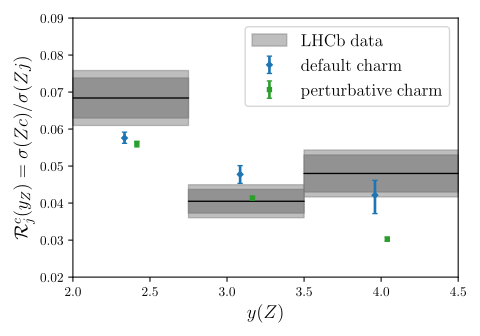
\includegraphics[width=.47\linewidth]{lhcb-zcharm-pheno.pdf}%
		\quad%
		\visible<2->{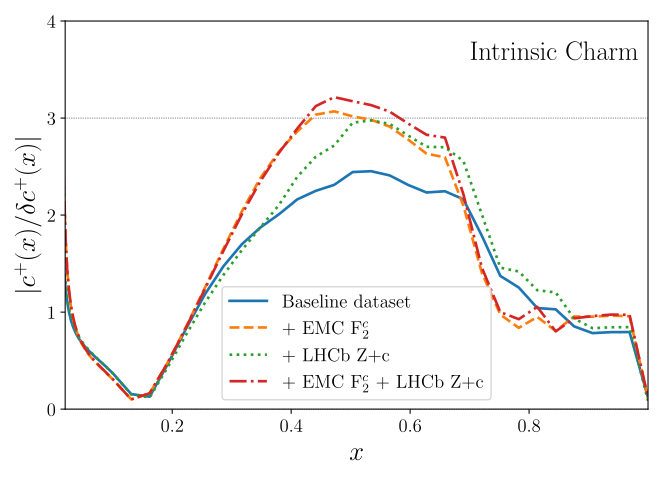
\includegraphics[width=.47\linewidth]{pull_baseline_EMC_LHCb_Zc.pdf}}
	\end{center}

	\begin{itemize}
		\item match better recent \textbf{LHCb} Z+c measurement \iRef{\href{https://doi.org/10.1103/PhysRevLett.128.082001}{PRL128-082001}}
		\item<2-> we find a $\bm{3\sigma}$ evidence of intrinsic charm
		\item<2-> result is \textbf{stable} with mass variation, dataset variation
	\end{itemize}
\end{frame}


\section{\yadism{} \iRef{in preparation}}

\begin{frame}{\yadism{} Physics Features}
	\begin{center}
		\includegraphics[width=.4\linewidth]{yadism.pdf}
	\end{center}

	\begin{itemize}
		\item DIS coefficient function database
		\item independent of boundary condition $\to$ \pdf{} fitting
		\item separate features: TMC, FNS, interpolation
		\item constant benchmark against \apfel{} (eventually discovering minor bugs there)
	\end{itemize}

	\vspace{10pt}
	same improvement in terms of project management as \eko{}!
\end{frame}

\begin{frame}{Coefficient Functions}
	\begin{itemize}
		\item implemented coefficient functions:
	\end{itemize}
	\begin{center}
		\begin{tabular}{l|l|l|l}
			& light & heavy & intrinsic\\\hline
			NC & $O(a_s^2)$ \iRef{\href{https://doi.org/10.1016/j.nuclphysb.2005.06.020}{VVM05},\href{https://doi.org/10.1016/j.physletb.2004.11.063}{MVV05},\href{https://doi.org/10.1016/S0550-3213(00)00045-6}{MV00}} & $O(a_s^2)$ \iRef{\href{https://arxiv.org/abs/1910.01536}{Hek19}} & $O(a_s)$ \iRef{\href{https://doi.org/10.1103/PhysRevD.58.094035}{KS98}}\\
			CC & $O(a_s^2)$ \iRef{\href{https://doi.org/10.1016/j.nuclphysb.2007.09.022}{MRV08},\href{https://doi.org/10.1016/j.nuclphysb.2009.01.001}{MVV09}} & $O(a_s)$ \iRef{\href{https://doi.org/10.1016/0370-2693(96)00456-X}{GKR96}} & $O(a_s)$ \iRef{in prep.}
		\end{tabular}
	\end{center}
	\begin{itemize}
		\item for CC intrinsic: see talk by K.~Kudashkin
		\item implemented flavor number schemes: \ffns{}, {\abbrev ZM-VFNS}, {\abbrev FONLL}
	\end{itemize}
\end{frame}

\begin{frame}{Comparison \yadism{} against \apfel{}}
	\begin{center}
		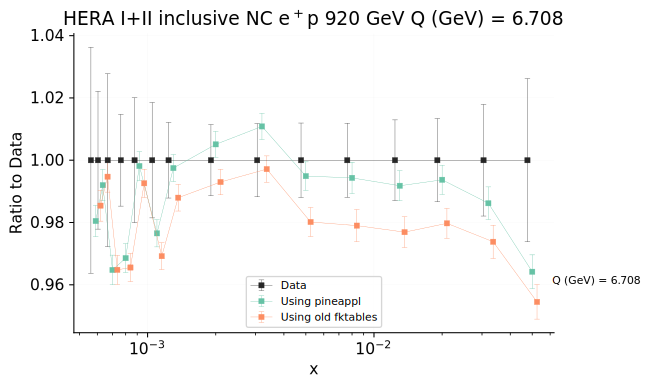
\includegraphics[width=.47\linewidth]{matched_datasets_from_dataspecs14_dataset_report_Datanorm_plot_fancy_dataspecs_11.pdf}%
		\quad%
		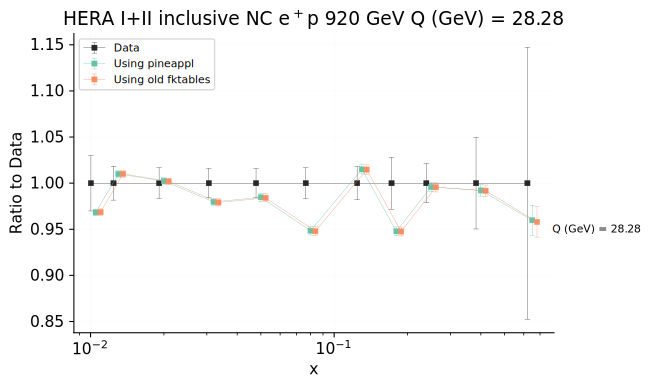
\includegraphics[width=.47\linewidth]{matched_datasets_from_dataspecs14_dataset_report_Datanorm_plot_fancy_dataspecs_23.pdf}

		\includegraphics[width=.47\linewidth]{matched_datasets_from_dataspecs4_dataset_report_Datanorm_plot_fancy_dataspecs_0.pdf}%
		\quad%
		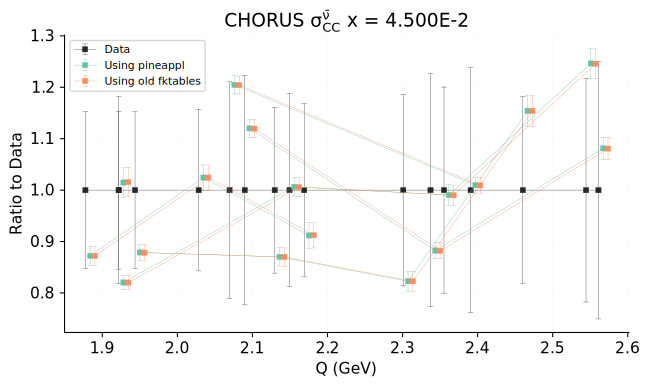
\includegraphics[width=.47\linewidth]{matched_datasets_from_dataspecs2_dataset_report_Datanorm_plot_fancy_dataspecs_0.pdf}

		{\color{vpGreen} green}, \enquote{pineappl} = \yadism{} vs. {\color{vpOrange} orange}, \enquote{old} = \apfel{}
	\end{center}
\end{frame}


\section{Theory Prediction Pipeline}

\begin{frame}{New Theory Prediction Pipeline}
	\begin{itemize}
		\item We're about to develop a new pipeline for theory predictions around \pineappl{} \iRef{\href{https://arxiv.org/abs/2008.12789}{arXiv:2008.12789}}
		\item both, \eko{} and \yadism{}, are interfaced with \pineappl{}
		\item \pineappl{} also has interfaces to {\abbrev mg5amc{\klammeraffe}nlo}, \appl{}, \fastnlo{}
		\item aim: produce \fk{} tables used in \pdf{} fitting
	\end{itemize}
\end{frame}


\begin{frame}[standout]
	Thank you!
\end{frame}

\end{document}
